%-----------------------------------------------------------------------------------------------------------------------------------------------%
%	The MIT License (MIT)
%
%	Copyright (c) 2021 Jitin Nair
%
%	Permission is hereby granted, free of charge, to any person obtaining a copy
%	of this software and associated documentation files (the "Software"), to deal
%	in the Software without restriction, including without limitation the rights
%	to use, copy, modify, merge, publish, distribute, sublicense, and/or sell
%	copies of the Software, and to permit persons to whom the Software is
%	furnished to do so, subject to the following conditions:
%	
%	THE SOFTWARE IS PROVIDED "AS IS", WITHOUT WARRANTY OF ANY KIND, EXPRESS OR
%	IMPLIED, INCLUDING BUT NOT LIMITED TO THE WARRANTIES OF MERCHANTABILITY,
%	FITNESS FOR A PARTICULAR PURPOSE AND NONINFRINGEMENT. IN NO EVENT SHALL THE
%	AUTHORS OR COPYRIGHT HOLDERS BE LIABLE FOR ANY CLAIM, DAMAGES OR OTHER
%	LIABILITY, WHETHER IN AN ACTION OF CONTRACT, TORT OR OTHERWISE, ARISING FROM,
%	OUT OF OR IN CONNECTION WITH THE SOFTWARE OR THE USE OR OTHER DEALINGS IN
%	THE SOFTWARE.
%	
%-----------------------------------------------------------------------------------------------------------------------------------------------%

%----------------------------------------------------------------------------------------
%	DOCUMENT DEFINITION
%----------------------------------------------------------------------------------------

% article class because we want to fully customize the page and not use a cv template
\documentclass[a4paper,10pt]{article}

%----------------------------------------------------------------------------------------
%	FONT
%----------------------------------------------------------------------------------------

% % fontspec allows you to use TTF/OTF fonts directly
% \usepackage{fontspec}
% \defaultfontfeatures{Ligatures=TeX}

% % modified for ShareLaTeX use
% \setmainfont[
% SmallCapsFont = Fontin-SmallCaps.otf,
% BoldFont = Fontin-Bold.otf,
% ItalicFont = Fontin-Italic.otf
% ]
% {Fontin.otf}

%----------------------------------------------------------------------------------------
%	PACKAGES
%----------------------------------------------------------------------------------------
\usepackage{url}
\usepackage{parskip} 	

%other packages for formatting
\RequirePackage{color}
\RequirePackage{graphicx}
\usepackage[usenames,dvipsnames]{xcolor}
\usepackage[scale=0.9]{geometry}

%tabularx environment
\usepackage{tabularx}

%for lists within experience section
\usepackage{enumitem}

% centered version of 'X' col. type
\newcolumntype{C}{>{\centering\arraybackslash}X} 

%to prevent spillover of tabular into next pages
\usepackage{supertabular}
\usepackage{tabularx}
\newlength{\fullcollw}
\setlength{\fullcollw}{0.47\textwidth}

%custom \section
\usepackage{titlesec}				
\usepackage{multicol}
\usepackage{multirow}

%CV Sections inspired by: 
%http://stefano.italians.nl/archives/26
\titleformat{\section}{\Large\scshape\raggedright}{}{0em}{}[\titlerule]
\titlespacing{\section}{0pt}{10pt}{10pt}

%for publications
\usepackage[style=authoryear,sorting=ynt, maxbibnames=2]{biblatex}

%Setup hyperref package, and colours for links
\usepackage[unicode, draft=false]{hyperref}
\definecolor{linkcolour}{rgb}{0,0.2,0.6}
\hypersetup{colorlinks,breaklinks,urlcolor=linkcolour,linkcolor=linkcolour}
\addbibresource{citations.bib}
\setlength\bibitemsep{1em}

%for social icons
\usepackage{fontawesome5}

%debug page outer frames
%\usepackage{showframe}

%----------------------------------------------------------------------------------------
%	BEGIN DOCUMENT
%----------------------------------------------------------------------------------------
\begin{document}

% non-numbered pages
\pagestyle{empty} 

%----------------------------------------------------------------------------------------
%	HEADING
%----------------------------------------------------------------------------------------

\begin{minipage}[c]{2.5cm}
    % 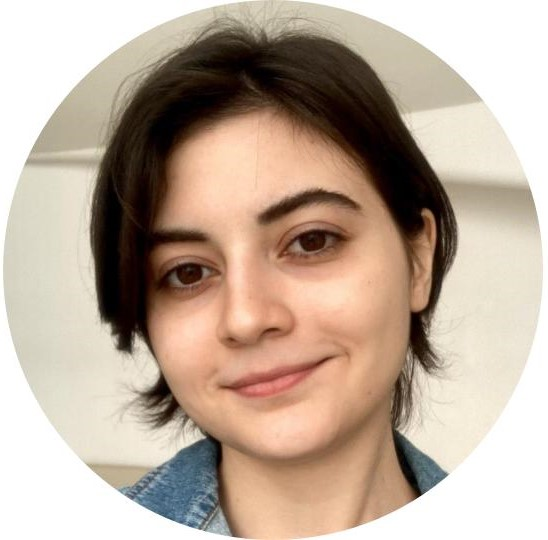
\includegraphics[width=2.5cm]{./avatar/avatar6.jpg}
\end{minipage}%
\hspace{0em} % bi aks
% \hspace{1em} % ba aks
\begin{minipage}[c]{\dimexpr\linewidth-2.5cm-15em\relax}
    \Huge{Arghavan Aslani}\\
    \vspace{0.1cm}\\
    \normalsize{M.Sc. student}
\end{minipage}%
\begin{minipage}[c]{0.3\linewidth}
    \href{https://github.com/arghavanaslani}{\raisebox{-0.05\height}\faGithub\ github.com/arghavanaslani} \\ 
    \href{https://www.linkedin.com/in/arghavan-aslani/}{\raisebox{-0.05\height}\faLinkedin\ arghavan-aslani} \\ 
    \href{mailto:aslaniarghavan@gmail.com}{\raisebox{-0.05\height}\faEnvelope \ aslaniarghavan@gmail.com} \\ 
    \href{tel:+989388687792}{\raisebox{-0.05\height}\faMobile \ +98.938.868.7792}
\end{minipage}

%----------------------------------------------------------------------------------------
%	EDUCATION
%----------------------------------------------------------------------------------------
\section{Education}

\begin{tabularx}{\linewidth}{@{}X r@{}}
    \textbf{M.Sc. in Cognitive Science, cog-SUP, Sorbonne Université and Université Paris Cité, Paris, France} & \textbf{2024 -} \\
    \multicolumn{2}{@{}X@{}}{\emph{Computational Neuroscience and Artificial Intelligence Track}} \\
    \href{https://cog-sup.fr/}{\raisebox{-0.05\height}\faGlobe\ cog-sup.fr} \\
\end{tabularx}

\begin{tabularx}{\linewidth}{@{}X r@{}}
    \textbf{B.Sc. in Electrical Engineering, University of Tehran, Tehran, Iran} & \textbf{2017 - 2022} \\
    \multicolumn{2}{@{}X@{}}{\emph{Control Systems Focus}} \\
\end{tabularx}

\begin{itemize}
    \item 
    \begin{tabularx}{\linewidth}{@{}X r@{}}
        Thesis: "LiveGaze: an integrated application for real-time gaze contingent display of multi-source eye-tracking data" & \href{https://github.com/arghavanaslani/livegaze}{Code Repository} \\
    \end{tabularx}
    \item 
    \begin{tabularx}{\linewidth}{@{}X r@{}}
        GPA: 15.24/20
    \end{tabularx}
\end{itemize}

% \begin{tabularx}{\linewidth}{@{}X r@{}}
%     \textbf{Mathematics and Physics Diploma, Farzanegan High School, Karaj, Alborz, Iran} & \textbf{2013 - 2017} \\
% \end{tabularx}

% \begin{itemize}
%     \item 
%     \begin{tabularx}{\linewidth}{@{}X r@{}}
%         GPA: 19.61/20
%     \end{tabularx}
% \end{itemize}

%----------------------------------------------------------------------------------------
% RESEARCH EXPERIENCE
%----------------------------------------------------------------------------------------

%Experience
\section{Research Experience}

\begin{tabularx}{\linewidth}{@{}X r@{}}
    \textbf{Crowd Cognition Group, Ludwig Maximilians Universität München —} & \hfill Apr. 2022 - present \\[3.75pt]
    \textbf{Research Assistant}\\
    \href{https://crowdcognition.net/}{\raisebox{-0.05\height}\faGlobe\ crowdcognition.net} \\
\end{tabularx}

\begin{tabularx}{\linewidth}{@{}X r@{}}
    \textbf{Co-supervisors: Dr. Bahador Bahrami, Prof. Ophelia Deroy}\\
\end{tabularx}

\begin{itemize}
    \item Data Analysis - Collaboration with Museu do Amanhã, Rio de Janeiro, Brazil
    \begin{itemize}
        \item Conducted a comprehensive analysis of eye-tracking data and questionnaires to address inquiries from museum stakeholders.
        \item Generated detailed reports, which included heatmaps, interactive diagrams, histograms of specific events from eye-tracking data, and identified meaningful patterns.
        \item Managed a team of 5 individuals, overseeing data collection and preprocessing.
    \end{itemize}
\end{itemize}

\begin{itemize}
    \item Investigating Variances in Visual Perception with Mobile Eye-Tracking
    \begin{itemize}
        \item Conducted data collection using the Pupil Invisible eye-tracking device in two conditions: individual and pair.
        \item Analyzed collected data with statistical tests, generated heatmaps, and applied various similarity metrics.       
    \end{itemize}
\end{itemize}

\begin{itemize}
    \item LiveGaze - Real-Time Visualization of Multi-Source Eye-Tracking Data
        \begin{itemize}
            \item Developed the MVP of the software using Pupil Invisible API, in Flask framework. The objective is to create real-time visualization including heatmaps and saliency maps from multiple observers.
            \end{itemize}
\end{itemize}

% \vspace{\baselineskip} 

\begin{tabularx}{\linewidth}{@{}X r@{}}
    \textbf{ESLAB, University of Tehran — Lead Reseach Assistant} & \hfill July 2021 - August 2022 \\[3.75pt]
    \href{https://www.linkedin.com/company/eng-sci-lab/}{\raisebox{-0.05\height}\faLinkedin\ www.linkedin.com/company/eng-sci-lab} \\
\end{tabularx}

\begin{tabularx}{\linewidth}{@{}X r@{}}
    \textbf{supervisor: Dr. Ehsan Maani Miandoab}\\
\end{tabularx}

\begin{tabularx}{\linewidth}{@{}X r@{}}
    {— Developed a 2-DOF robot named "Spider-Paint" capable of translating images into drawings on a whiteboard using a marker.} \href{https://github.com/arghavanaslani/spider-paint/blob/'spider-paint'/README.md}{(Link to Videos)} \\[3.75pt]
    {— Designed and implemented a control algorithm in C to operate two stepper motors on a vertical plane using a single Arduino.} \href{https://github.com/arghavanaslani/spider-paint}{(Link to Code)} \\[3.75pt]
    {— Authored a paper accepted at the ISME Conference 2022 by consolidating contributions from various team members.}
\end{tabularx}

% \vspace{\baselineskip} 

%----------------------------------------------------------------------------------------
%	PUBLICATIONS
%----------------------------------------------------------------------------------------

\section{Publications}

\begin{itemize}
    \item \textbf{Screens in the Museum: Understanding Visitor Interactions Through Mobile Eye-Tracking}\\
    Contributors: \textbf{A. Aslani}, S. Saeedpour, D. Ferreiro, B. Bahrami, O. Deroy\\
    Status: Under Preparation
\end{itemize}

\begin{itemize}
    \item \textbf{Measuring Gaze Scan-Path Similarity Between Observers Using Mobile Eye-Tracking}\\
    Contributors: D. Gulhan, A. Aliyeva, \textbf{A. Aslani}, O. Deroy, B. Bahrami\\
    Status: Under Preparation
\end{itemize}


\begin{itemize}
    \item \textbf{Design, Fabrication and Control of 2 DoF Robot in Vertical Plane}\\
    Authors: \textbf{A. Aslani}, E. Maani Miandoab, H. Najafi, H. Bahreininan, M. Hemmati, M. Fakher\\
    Conference: The 30th Annual International Conference of the Iranian Society of Mechanical Engineers, 2022\\
    Publisher:  \href{https://civilica.com/doc/1468825/}{https://civilica.com/doc/1468825/}
\end{itemize}

% \vspace{\baselineskip} 



%----------------------------------------------------------------------------------------
% WORK EXPERIENCE
%----------------------------------------------------------------------------------------

\section{Work Experience}

\begin{tabularx}{\linewidth}{@{}X r@{}}
    \textbf{CLIC, University of Tehran — Market Analyst} & \hfill July 2019 - Sep 2019 \\[3.75pt]
\end{tabularx}

\begin{tabularx}{\linewidth}{@{}X r@{}}
    {— Analyzed the product's value propositions, estimated market size, and identified early adopters to pinpoint optimal markets for eye-tracking devices.}\\
    {— Scheduled and facilitated meetings with potential customers from major companies to understand their needs.}\\
\end{tabularx}

%----------------------------------------------------------------------------------------
% EPROJECTS
%----------------------------------------------------------------------------------------

%Projects
\section{Projects}

\begin{tabularx}{\linewidth}{ @{}l r@{} }
    \textbf{Exploratory Analysis of Digikala User Search Data} & \\[3.75pt]
    \multicolumn{2}{@{}X@{}}{Conducted in-depth exploratory analysis on user search data from Digikala, Iran's largest online retailer, based on the previous year's dataset. Due to confidentiality, the analysis was performed in a secure environment, and the specific details and notebook cannot be shared.}  \\
\end{tabularx}

\begin{tabularx}{\linewidth}{ @{}l r@{} }
    \textbf{User Experience Analysis for Language Learning App (Alpha)} & \\[3.75pt]
    \multicolumn{2}{@{}X@{}}{Lead the user experience data collection and analysis initiative for the alpha version of a language learning application. Employing surveys, interviews, and user behavior analytics to gather insights aimed at enhancing usability and addressing user needs effectively.}  \\
\end{tabularx}

% \begin{tabularx}{\linewidth}{ @{}l r@{} }
%     \textbf{Web Scraping for Job Advertisements in https://jobvision.ir} & \hfill \href{https://github.com/arghavanaslani/JobAdDB}{Link to Code} \\[3.75pt]
%     \multicolumn{2}{@{}X@{}}{Developed in Python.
%     Utilized BeautifulSoup, pandas, and requests for web scraping and data processing.
%     Created a custom database due to the unavailability of existing datasets in the field.}  \\
% \end{tabularx}

%----------------------------------------------------------------------------------------
%	ADDITIONAL TRAINING
%----------------------------------------------------------------------------------------
\section{Additional Training}

\begin{tabularx}{\linewidth}{ @{}l X r@{} }
    \textbf{Computational Neuroscience Boot Camp, Neuromatch Academy} & & \hfill \href{https://portal.neuromatchacademy.org/certificate/ee23deef-9e73-4233-8c46-6e85375d9f1b}{Certificate} \\[3.75pt]
    % \textbf{Data Analysis Program, Karyar College} \\ {             Karyar is a social startup aimed at training skilled software developers.} \\ {              I was granted a scholarship by Digikala, Iran's largest online retailer, to take this program.} \\
    \textbf{Task-Oriented Course in Data Analysis with Python} & & \hfill \href{https://quera.org/certificate/7p1aeaOn/}{Certificate} \\[3.75pt]
    \textbf{Task-Oriented Course in SQL} & & \hfill \href{https://quera.org/certificate/D4uYyhcQ/}{Certificate} \\
\end{tabularx}

%----------------------------------------------------------------------------------------
%	 Extracurricular Activities
%----------------------------------------------------------------------------------------
\section{Extracurricular Activities}

\begin{itemize}
    \item 
    \begin{tabularx}{\linewidth}{@{}X r@{}}
        {Member of BTCS (Brain Tech and Cognitive Science Club)}\\
    \end{tabularx}
    Contributed to event planning and execution to attract students to the field.
    \item 
    \begin{tabularx}{\linewidth}{@{}X r@{}}
        {Performer and Member of Council at Performing Arts Club} & \hfill \href{https://www.instagram.com/fanni_theater/}{Link to Instagram Page} \\[3.75pt]
    \end{tabularx}
\end{itemize}

%----------------------------------------------------------------------------------------
%	LANGUAGES
%----------------------------------------------------------------------------------------
\section{Languages}
\begin{tabularx}{\linewidth}{@{}l X@{}}
    English &  \normalsize{Full Professional Proficiency (IELTS overall:7.5, L:8.5, R:7.5, W:7, S:7.5)}\\
    Farsi(Persian) &  \normalsize{Native or bilingual proficiency}\\
    % Turkish &  \normalsize{Limited working proficiency}\\  
    % Arabic &  \normalsize{Elementary proficiency}\\ 
    
\end{tabularx}

%----------------------------------------------------------------------------------------
%	SKILLS
%----------------------------------------------------------------------------------------
\section{Technical Skills}
\begin{tabularx}{\linewidth}{@{}l X@{}}
    Data Analysis &  \normalsize{Python (Numpy, Pandas, Matplotlib, Seaborn, scikit-learn), SQL (Postgres, MySQL), MATLAB, R}\\
    Web Development &  \normalsize{Python (Flask, Django), HTML5, CSS, JavaScript}\\
    Operating Systems &  \normalsize{Linux(Ubuntu), Windows}\\  
    Tools &  \normalsize{Git, Jupyter Notebook, LATEX, Microsoft Office}\\ 
    
\end{tabularx}



%----------------------------------------------------------------------------------------
%	REFERENCES
%----------------------------------------------------------------------------------------

\section{References}

\begin{itemize}
    \item \textbf{Dr. Bahador Bahrami} - \href{mailto:bahador.bahrami@psy.lmu.de}{bahador.bahrami@psy.lmu.de}\\
    Director of Crowd Cognition Lab, Faculty of Psychology and Educational Sciences, Ludwig Maximilian University, Munich
    \item \textbf{Prof. Ophelia Deroy} - \href{mailto:Ophelia.Deroy@lrz.uni-muenchen.de}{Ophelia.Deroy@lrz.uni-muenchen.de}\\
    Chair for Philosophy of Mind and Neuroscience, Ludwig Maximilian University, Munich
    \item \textbf{Dr. Ehsan Maani Miandoab} - \href{mailto:e.maani@ut.ac.ir}{e.maani@ut.ac.ir}\\
    Assistant Professor, Faculty of Engineering Sciences, College of Engineering, University of Tehran, Iran

\end{itemize}


\end{document}
